%\documentclass[journal]{IEEEtran}
%\documentclass[12pt,onecolumn]{IEEEtran}
\documentclass[UTF8]{article}
\usepackage{ctex}
\usepackage{geometry,graphicx,marvosym}
\usepackage{amsmath,amsthm}
\usepackage{amsfonts}
\usepackage[usenames,dvipsnames]{pstricks}
\usepackage{pst-plot,pstricks-add}
%\usepackage{graphicx,times,amsmath,amssymb,multirow,subfigure}
\usepackage{graphicx,times,amsmath,amssymb,multirow}
\usepackage{url}
\usepackage{stfloats}
\usepackage{amsfonts,rotating}
\usepackage{color}
\usepackage{verbatim,multirow}
% setting dimension of the paper
\textwidth 7.0true in
\textheight 8.9 true in
\topmargin=-20pt
\headheight=6pt
\headsep=2pt
\oddsidemargin -0.3true in
\evensidemargin -0.4true in
\usepackage{amssymb}

\newtheorem{theorem}{Theorem}
\newtheorem{lemma}{Lemma}
\newtheorem{algorithm}{Algorithm}
\newtheorem{definition}{Definition}
\newtheorem{proposition}{Proposition}

\newcommand{\dtcwt}{\operatorname{DT-\mathbb{C}WT}}
\newcommand{\tpctf}{\operatorname{TP-\mathbb{C}TF}}
\newcommand{\ctf}{\operatorname{\mathbb{C}TF}}
\newcommand{\tr}[1]{\textcolor{red}{#1}}
\newcommand{\tb}[1]{\textcolor{blue}{#1}}
\newcommand{\mO}{{\mathcal{T}}}
\newcommand{\C}{\mathbb{C}}    %complex number field
\newcommand{\N}{\mathbb{N}}    %natural numbers
\newcommand{\R}{\mathbb{R}}    %real number field
\newcommand{\Z}{\mathbb{Z}}    %integers
\newcommand{\imag}{\mathrm{i}} % imaginary unit
\newcommand{\dR}{\mathbb{R}^d}
\newcommand{\dT}{\mathbb{T}^d}
\newcommand{\dZ}{\mathbb{Z}^d}
\newcommand{\dlp}[1]{l_{#1}(\mathbb{Z}^d)}
\newcommand{\td}{\boldsymbol{\delta}}  %Dirac/Kronicker sequence
\newcommand{\bp}{\begin{proof}}
	\newcommand{\ep}{\hfill  \end{proof} }
\newcommand{\be}{ \begin{equation} }
	\newcommand{\ee}{ \end{equation} }
\newcommand{\dLp}[1]{L_{#1}(\mathbb{R}^d)}
\newcommand{\prm}{P}           %projection matrix
\newcommand{\wh}{\widehat}
\renewcommand{\le}{\leqslant}
\renewcommand{\ge}{\geqslant}
\newcommand{\bs}{\backslash}
\newcommand{\ol}{\overline}
\newcommand{\vk}{\mathsf{k}}
\newcommand{\la}{\langle}
\newcommand{\ra}{\rangle}
\newcommand{\tp}{\mathsf{T}}  %transpose
\newcommand{\conj}{\overline}
\newcommand{\supp}{\mathrm{supp}}
\newcommand{\setsp}{\;:\;}     %set separator
\newcommand{\sd}{\mathcal{S}}  %subdivision operator S
\newcommand{\tz}{\mathcal{T}}  %transition operator T
\newcommand{\wt}{\widetilde}
\renewcommand{\le}{\leqslant}
\renewcommand{\ge}{\geqslant}
\newcommand{\er}{\eqref}
\newcommand{\gep}{\varepsilon}
\newcommand{\eps}{\epsilon}
\newcommand{\gl}{\lambda}
\newcommand{\gL}{\Lambda}
\newcommand{\gd}{\delta}
\newcommand{\DAS}{\mathrm{DAS}}
\newcommand{\UDAS}{\mathrm{UDAS}}
\newcommand{\DHF}{\mathrm{DHF}}
\newcommand{\bm}{\boldmath}
\newtheorem{example}{Example}
\bibliographystyle{unsrt}
\newcommand{\xz}[1]{\textcolor{magenta}{\bf #1}}
\usepackage[colorlinks,linkcolor=blue,anchorcolor=blue,citecolor=blue]{hyperref}
\usepackage{indentfirst}
\usepackage{subcaption}

\usepackage{geometry}
\geometry{a4paper,scale=0.8}
\boldmath
\begin{document}
	\author{Huang Yijun}
\title{Report : Exploiting 3D Framlets to Extract Structrual Sparsity from Image and Coil Images}
\maketitle

\section{Notation definition}
\begin{enumerate}
	\item $u$ : the desired MRI image.
	\item $g$ : the measured $k$-space data.
	\item $S$ : the coil sensitivity matrix.
	\item $F$ : the discrete Fourier transform matrix.
	\item $P$ : the undersampled mask.
	\item $\tilde{P}$ : the undersampled mask opposite to $P$.
	\item $W$ : the 3D tight framelet transform matrix.
\end{enumerate}

\section{The MRI reconstruction model}
\par The 3D framelet regularization MRI model:
\begin{equation} \label{model}
	min \left\{ \frac{1}{2} \Vert Mu-g \Vert_2^2 + \Vert \Gamma W (A u + G)\Vert_1  \right\}
\end{equation}
where $M$ denotes $PFS$, $A$ and $G$ is given by
\begin{equation}
	A = \begin{bmatrix}
		I & 0 \\
		0 & F^{-1}\tilde{P}FS
	\end{bmatrix}
	\qquad
 	G = \begin{bmatrix}
 		0 \\
 		F^{-1}g \\
 	\end{bmatrix}
\end{equation}
The first term in (\ref{model}) is data fidelity term  while the second term extracts the structrual sparsity from the image and coil images, and the proposed model (\ref{model}) can be solved by PD3O.

\section{The structrual sparsity from image and coil images}
\par In this section, we explore the structrual sparsity from image and coil images using 3D tight framelet. The full sampled image and its coil images are depicted in Fig \ref{images}, then we can stack the all images to  form a 3D structure. Consequently,  the 3D tight framelet transfrom can be performed on this 3D image structure. The fifth high pass coefficients under the 3D transform is showed in Fig \ref{coefs}. 
\begin{figure}[ht]
	
	\centering
	\begin{subfigure}[t]{0.15\textwidth}
		\centering
		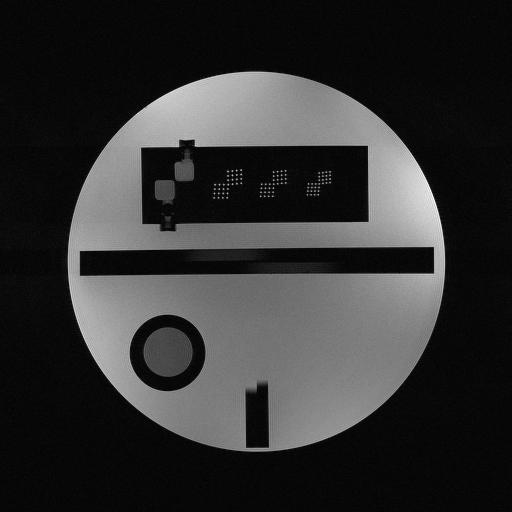
\includegraphics[width=\textwidth]{./image/full.jpg}
		\caption{full-sampled image}
		\label{fig:1a}
	\end{subfigure}
	\begin{subfigure}[t]{0.15\textwidth}
		\centering
		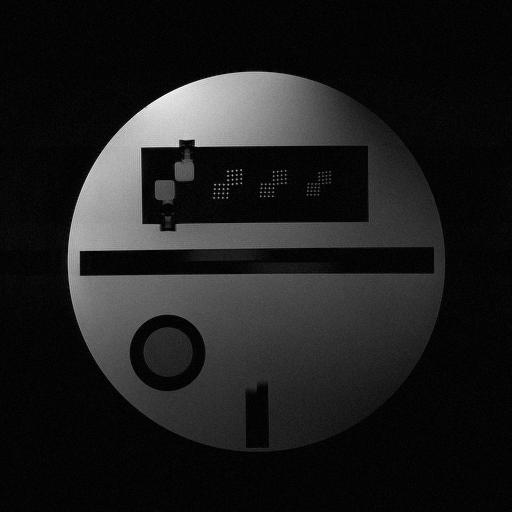
\includegraphics[width=\textwidth]{./image/1coil.jpg}
		\caption{coil 1 }
		\label{fig:1b}
	\end{subfigure}
	\begin{subfigure}[t]{0.15\textwidth}
		\centering
		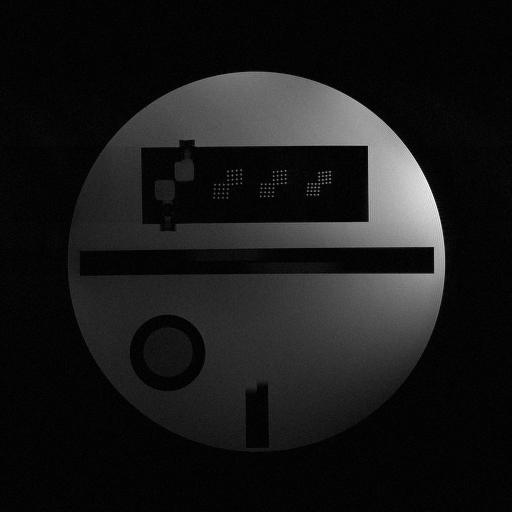
\includegraphics[width=\textwidth]{./image/2coil.jpg}
		\caption{coil 2 }
		\label{fig:1c}
	\end{subfigure}
	\begin{subfigure}[t]{0.15\textwidth}
		\centering
		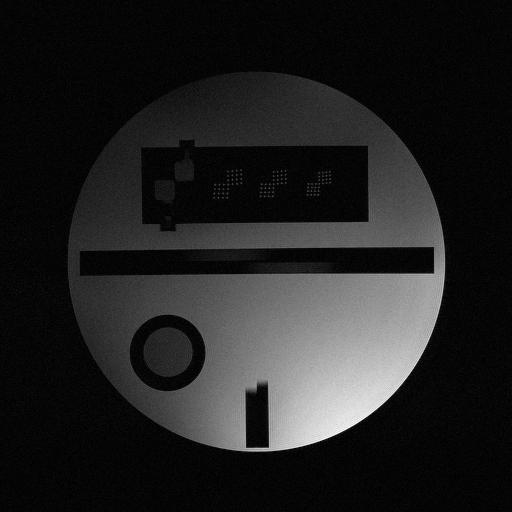
\includegraphics[width=\textwidth]{./image/3coil.jpg}
		\caption{coil 3 }
		\label{fig:1d}
	\end{subfigure}
	\begin{subfigure}[t]{0.15\textwidth}
		\centering
		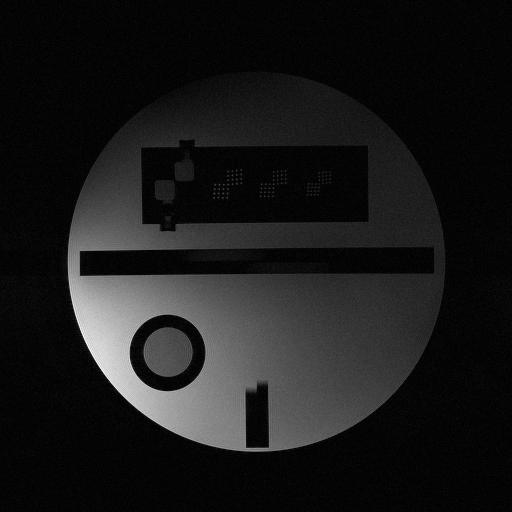
\includegraphics[width=\textwidth]{./image/4coil.jpg}
		\caption{coil 4 }
		\label{fig:1e}
	\end{subfigure}
	\caption{full image and its four coil images}
	\label{images}
\end{figure}
\par Fig \ref{fig:2a}-\ref{fig:2e} are the xy-plane coeffiecients under the transform, which extracted from the image and coil images, while the Fig \ref{fig:3b}-\ref{fig:3e} are extracted from coil images. From the decomposition results, the feature extracted from the image and coil images is better than those extracted from coil images only. 
\begin{figure}[ht]
	\centering
	\begin{subfigure}[h]{0.2\textwidth}
		\centering
		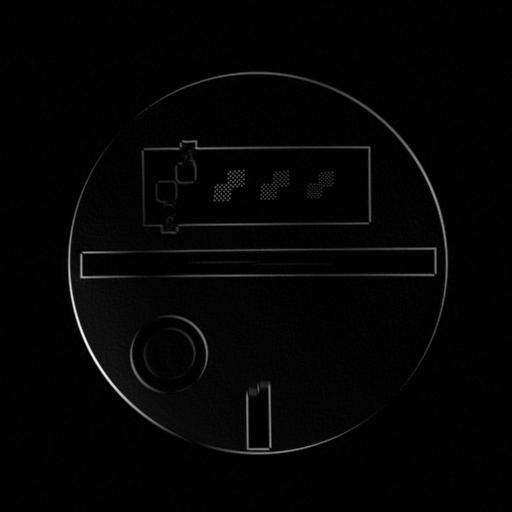
\includegraphics[scale=0.15]{./image/1c.jpg}
		\caption{full-sampled image}
		\label{fig:2a}
	\end{subfigure}

	\begin{subfigure}[h]{0.2\textwidth}
		\centering
		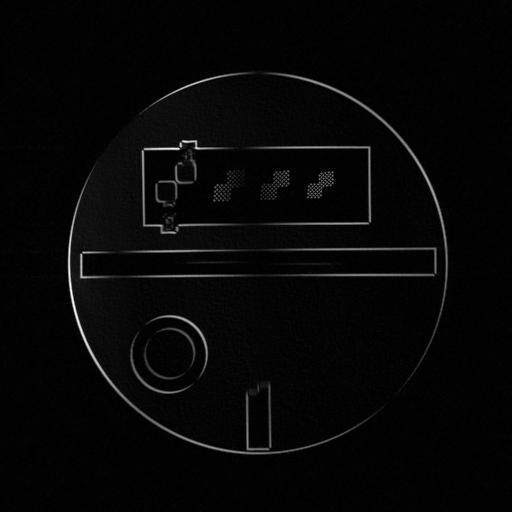
\includegraphics[scale=0.15]{./image/2c.jpg}
		\caption{coil 1 }
		\label{fig:2b}
	\end{subfigure}
	\begin{subfigure}[h]{0.2\textwidth}
		\centering
		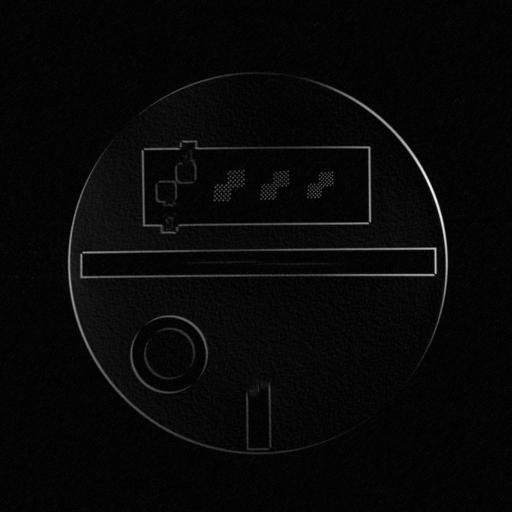
\includegraphics[scale=0.15]{./image/3c.jpg}
		\caption{coil 2 }
		\label{fig:2c}
	\end{subfigure}
	\begin{subfigure}[h]{0.2\textwidth}
		\centering
		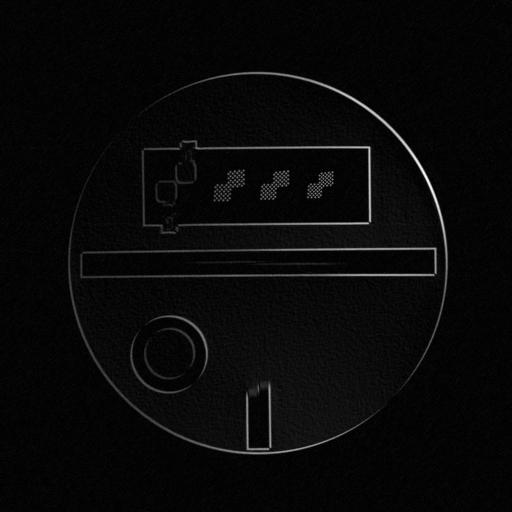
\includegraphics[scale=0.15]{./image/4c.jpg}
		\caption{coil 3 }
		\label{fig:2d}
	\end{subfigure}
	\begin{subfigure}[h]{0.2\textwidth}
		\centering
		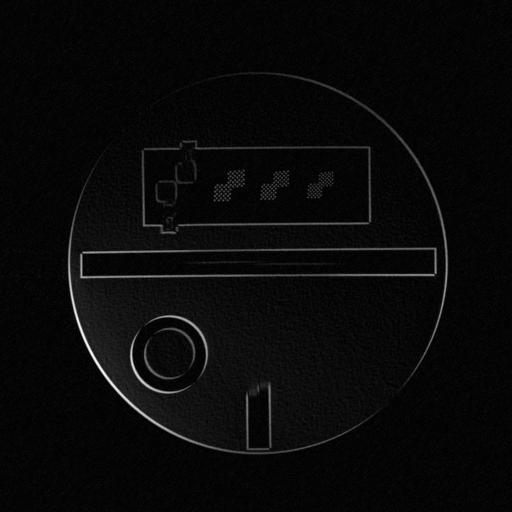
\includegraphics[scale=0.15]{./image/5c.jpg}
		\caption{coil 4 }
		\label{fig:2e}
	\end{subfigure}\\
	%% coefficents
	\begin{subfigure}[h]{0.2\textwidth}
		\centering
		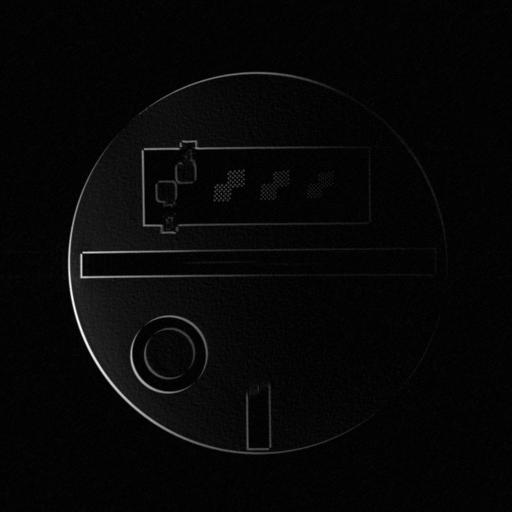
\includegraphics[scale=0.15]{./image/1cc.jpg}
		\caption{coil 1 }
		\label{fig:3b}
	\end{subfigure}
	\begin{subfigure}[h]{0.2\textwidth}
		\centering
		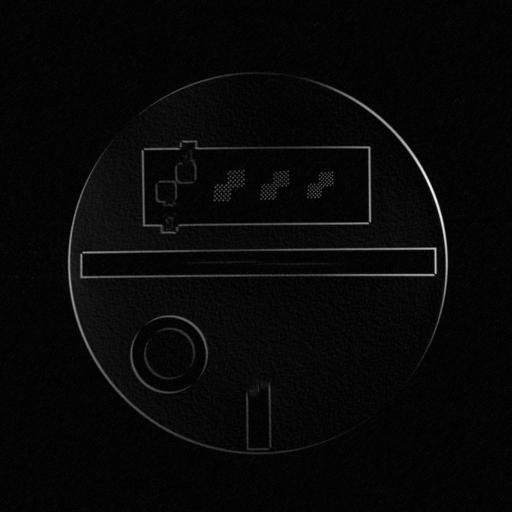
\includegraphics[scale=0.15]{./image/2cc.jpg}
		\caption{coil 2 }
		\label{fig:3c}
	\end{subfigure}
	\begin{subfigure}[h]{0.2\textwidth}
		\centering
		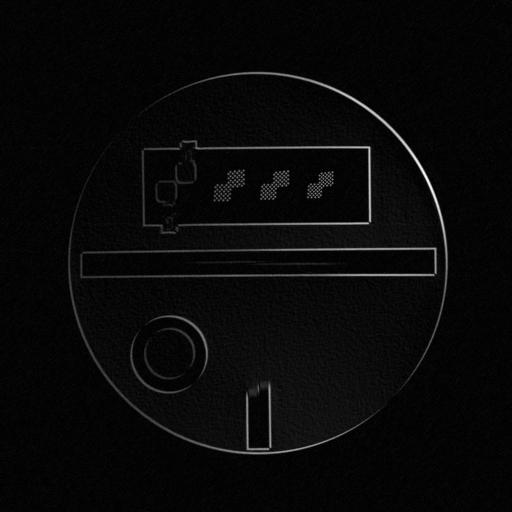
\includegraphics[scale=0.15]{./image/3cc.jpg}
		\caption{coil 3 }
		\label{fig:3d}
	\end{subfigure}
	\begin{subfigure}[h]{0.2\textwidth}
		\centering
		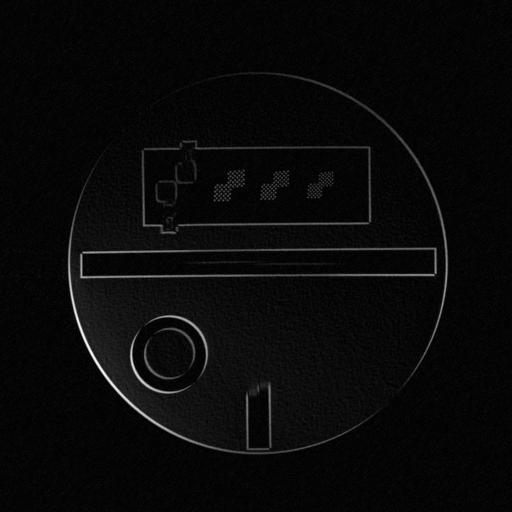
\includegraphics[scale=0.15]{./image/4cc.jpg}
		\caption{coil 4 }
		\label{fig:3e}
	\end{subfigure}
	\caption{The fifth high pass coefficients under the 3D transform(xy-plane). (a)-(e):The 3D transform is performed on the image and its coil images; (f)-(i) The 3D transform is performed on the coil images}
	\label{coefs}
\end{figure}


\section{Numerical algorithm}
\par For solving the model (\ref{model}), define the function $f(u) = \frac{1}{2}\Vert Mu-g \Vert_2^2 $ and $h(u) = \Vert \Gamma(u+b) \Vert_1$, therefore the model (\ref{model}) can be rewritten as
\begin{equation}
	min \left\{ f(u) + h(Bu)  \right\} 
\end{equation}
where the $B=WA$ and $b = WG$.
\par Based on the above description, the algorithm is written as follows : given the initial guess$(v^0, z^0)$ and parameters $\gamma$, $\delta$ and $\Gamma$, it iterates

\begin{equation*}
	\begin{cases}
	 u^k = real(v^k) \\
	 \omega^k = (I-\gamma \delta BB^T)z^k + \delta B(\bar{v^k} - \gamma \nabla f(u^k))\\
	 z^k = ( \omega^k+\delta b) - soft(\omega^k+\delta b, \Gamma) \\
	 v^{k+1} = u^k - \gamma \nabla f(u^k) - \gamma B^T z^{k+1}
	\end{cases}
\end{equation*}
\end{document}